\PassOptionsToPackage{dvipsnames,svgnames,table}{xcolor}
\documentclass[10pt]{article}
\usepackage[a4paper,margin=22mm]{geometry}
\usepackage[no-math]{fontspec}\setmainfont[SmallCapsFont={Latin Modern Roman Caps}]{Latin Modern Roman}
\usepackage{amsmath,amssymb,amsthm,mathtools,graphicx,xcolor,hyperref,xurl,xspace,ifthen,enumerate,textcomp}
\usepackage[shortlabels]{enumitem}
\setlength{\emergencystretch}{4em}
\usepackage{aliascnt}
\usepackage[capitalize]{cleveref}
\newtheorem{theorem}{Theorem}[section]
\newtheorem{theo}[theorem]{Theorem}
\newtheorem{thm}[theorem]{Theorem}
\newaliascnt{lemma}{theorem}
\newtheorem{lemma}[lemma]{Lemma}
\aliascntresetthe{lemma}
\newtheorem{lemm}[theorem]{Lemma}
\newtheorem{prop}[theorem]{Proposition}
\newtheorem{coro}[theorem]{Corollary}
\newtheorem{corollary}[theorem]{Corollary}
\newtheorem{fact}[theorem]{Fact}
\newtheorem{claim}[theorem]{Claim}
\theoremstyle{definition}
\newtheorem{defi}[theorem]{Definition}
\newtheorem{definition}[theorem]{Definition}
\newtheorem{rema}[theorem]{Remark}
\newtheorem{remark}[theorem]{Remark}
\newtheorem{exam}[theorem]{Example}
\newtheorem{example}[theorem]{Example}
\newenvironment{enonce*}[2][]{\par\medskip\noindent\textbf{#2.}\itshape}{\par\medskip}
\providecommand{\eg}{e.g.\ }
\providecommand{\ie}{i.e.\ }
\providecommand{\resp}{resp.\ }
\providecommand{\cf}{cf.\ }
\providecommand{\longthanks}[1]{\par\smallskip\noindent #1\par\smallskip}
\usepackage{mathrsfs}
\usepackage{tikz}
\usetikzlibrary{patterns}
%

 %


\crefname{coro}{Corollary}{Corollaries}
\crefname{defi}{Definition}{Definitions}
\crefname{lemm}{Lemma}{Lemmas}
\crefname{prop}{Proposition}{Propositions}
\crefname{rema}{Remark}{Remarks}
\crefname{theo}{Theorem}{Theorems}
%
%
\newcommand{\creflastconjunction}{, and\nobreakspace} %



\newcommand{\ZZ}{\mathbb{Z}}


\newcommand{\ov}[1]{\overline{#1}}

\newcommand{\oeis}[1]{\href{https://oeis.org/#1}{{#1}}}

\newcommand{\defin}[1]{\emph{\color{red}{#1}}}

\newcommand{\level}{\mathscr{L}}
\newcommand{\Dyck}{\mathscr{D}}
\newcommand{\mono}{\overline{\mathbb{M}}_1}
\newcommand{\monod}{\mathbb{M}_1}
\newcommand{\monoi}{\mathbb{M}_2}
\newcommand{\sm}{\leq}
\newcommand{\wmin}{w_{\min}}
\newcommand{\pscolle}{\ast}
\newcommand{\colle}{\,\sharp\,}
\newcommand{\deri}{\mathsf{D}}

\DeclareMathOperator{\up}{Up}
\DeclareMathOperator{\des}{Desc}
\DeclareMathOperator{\rise}{Rise}
\crefname{lemma}{Lemma}{Lemmas}
\begin{document}
\section*{1507. Meet-semilattice structure and a prefix-refining meet algorithm for the movable-block Dyck-path order}
Chapoton, Frédéric. \emph{Some properties of a new partial order on Dyck paths}. Algebraic Combinatorics 3 (2020), publisher version, DOI 10.5802/alco.98. \url{https://alco.centre-mersenne.org/articles/10.5802/alco.98/}. CC BY4.0.
\paragraph{Selected problem and scope (editorial).} Exact original Theorem7.6 for the source-defined movable-block Dyck-path order is selected. All native Section1 notation, movement conventions and Hasse illustration, plus the complete Section7 locked/unlocked block decomposition, rise operators, replay/overlap cases, prefix cofinality, maximal descent and terminal meet construction are retained. The one imported support sketch is an exact bounded unlabeled graphical illustration from the same licensed publishedPDF; every general formula, diagram label and human proof is native editable TeX. No source-local meet construction is taken as a prerequisite, and no Tamari, enumerative or principal-ideal variant is counted.
\paragraph{Difficulty (editorial).} The proof must construct the unique prefix-compatible rise minimum and descent maximum for the author-specific movable-block order, including the full nested/overlapping slide cases at native1560–1691 and1742–1808. These constructions then preserve the entire common-lower-set while strictly increasing the shared prefix, yielding the meet by termination at1834–1864. No named external lattice theorem supplies this new local order mechanism; the single meet-semilattice outcome is proposed as H2.
\paragraph{Formatting (editorial).} Exact human-authored mathematical text, formulas and proof order are retained in source order. Only standalone typography/front matter, original counter restoration, bibliography presentation and the declared noncore printed reference locators are adapted. Non-rendered author comments are excluded while every percent newline guard is retained. No mathematical argument, correction or reconstruction is generated.
\clearpage

\section{Construction and first properties}

In this section, after recalling some notations, the partial order
$\Dyck_n$ is defined through its Hasse diagram. Some properties of
this partial order are proved.

\label{sec1}
A \defin{Dyck path} of size $n \geq 0$ is a lattice path from $(0,0)$ to
$(2 n,0)$ using only north-east and south-east steps and staying weakly above
the horizontal line.

We will also consider Dyck paths of size $n$ as words of length $2 n$
in the alphabet $\{0,1\}$, where $1$ stands for a north-east step and
$0$ for a south-east step.

\begin{figure}[htb]\centering
\begin{tikzpicture}[scale=0.2]
\draw[gray,very thin] (0, 0) grid (48, 8);  
\draw[rounded corners=1, color=black, line width=2] (0, 0) -- (1, 1) -- (2, 2) -- (3, 3) -- (4, 4) -- (5, 3) -- (6, 4) -- (7, 5) -- (8, 4) -- (9, 3) -- (10, 4) -- (11, 5) -- (12, 4) -- (13, 3) -- (14, 2) -- (15, 1) -- (16, 2) -- (17, 1) -- (18, 0) -- (19, 1) -- (20, 2) -- (21, 1) -- (22, 2) -- (23, 3) -- (24, 2) -- (25, 3) -- (26, 4) -- (27, 3) -- (28, 4) -- (29, 5) -- (30, 6) -- (31, 5) -- (32, 6) -- (33, 5) -- (34, 6) -- (35, 7) -- (36, 8) -- (37, 7) -- (38, 6) -- (39, 5) -- (40, 4) -- (41, 5) -- (42, 4) -- (43, 3) -- (44, 2) -- (45, 1) -- (46, 0) -- (47, 1) -- (48, 0);
\end{tikzpicture}
\caption{A typical example}
\label{typique}
\end{figure}
\Cref{typique} displays a typical example.

The \defin{area} under a Dyck path is the surface of the domain between
the horizontal line and the Dyck path.

Every Dyck path can be uniquely written as the concatenation of
several blocks, where in every block the only vertices on the
horizontal line are the first and last ones. If there is only one
block, the Dyck path is said to be \defin{block-indecomposable}. The
example displayed above has $3$ blocks.

Inside a Dyck path, a subsequence of consecutive steps is called a
\defin{subpath} if it starts and ends at the same height and keeps
strictly above that height in between. Here the height is the
vertical coordinate, increased by north-east steps and decreased by
south-east steps.

Let us say that a subpath $x$ of a Dyck path $w$ is \defin{movable} if
it is preceded in $w$ by the letter $0$ and
\begin{itemize}
\item either $x$ ends at the last letter of $w$,
\item or $x$ is followed in $w$ by the letter $1$.
\end{itemize}

\begin{figure}[htb]\centering
\begin{minipage}[b]{0.5\textwidth}\centering
\begin{tikzpicture}[scale=0.35]
  \draw[gray,very thin] (0, 0) grid (10, 2);
  \draw[rounded corners=1, color=black, line width=2] (0, 0) -- (1, 1) -- (2, 0) -- (3, 1) -- (4, 2) -- (5, 1) -- (6, 2) -- (7, 1) -- (8, 0) -- (9, 1) -- (10, 0);
  \draw[rounded corners=1, pattern=north west lines, pattern color=teal] (5, 1) -- (6, 2)-- (7, 1) ;
\end{tikzpicture}
\caption{A subpath which is not movable.}\end{minipage}\hfill
\begin{minipage}[b]{0.45\textwidth}\centering
\begin{tikzpicture}[scale=0.35]
  \draw[gray,very thin] (0, 0) grid (10, 2);
  \draw[rounded corners=1, color=black, line width=2] (0, 0) -- (1, 1) -- (2, 0) -- (3, 1) -- (4, 2) -- (5, 1) -- (6, 2) -- (7, 1) -- (8, 0) -- (9, 1) -- (10, 0);
  \draw[rounded corners=1, pattern=north west lines, pattern color=teal] (2, 0) -- (3, 1) -- (4, 2) -- (5, 1) -- (6, 2) -- (7, 1) -- (8, 0);
\end{tikzpicture}\caption{A movable subpath.}\end{minipage}\hfill

\vspace*{5mm}
\begin{minipage}[b]{0.45\textwidth}\centering
\begin{tikzpicture}[scale=0.35]
  \draw[gray,very thin] (0, 0) grid (10, 2);
  \draw[rounded corners=1, color=black, line width=2] (0, 0) -- (1, 1) -- (2, 0) -- (3, 1) -- (4, 2) -- (5, 1) -- (6, 2) -- (7, 1) -- (8, 0) -- (9, 1) -- (10, 0);
  \draw[rounded corners=1, pattern=north west lines, pattern color=teal] (8, 0) -- (9, 1) -- (10, 0);
\end{tikzpicture}\caption{A movable subpath.}\end{minipage}
\end{figure}

For every Dyck path $w$ and every movable subpath $x$ in $w$, let
$N(w,x)$ be the number of consecutive $0$ letters that appear just
before $x$. For any integer $1 \leq i \leq N(w,x)$ (corresponding to a
choice among the consecutive $0$ letters just before $x$), let us
define another Dyck path $M(w,x,i)$ as the following word:
\begin{itemize}
\item first the initial part of $w$ until the letter before the chosen $0$,
\item then $x$,
\item then the $0$ letters starting at the chosen $0$,
\item then the final part of $w$ after $x$.
\end{itemize}
Graphically, this transformation corresponds to sliding the
subpath $x$ in the north-west direction by one or several steps.

%

\begin{figure}[htb]\centering
\begin{tikzpicture}[scale=0.4]  
\draw[gray,very thin] (0, 0) grid (12, 3);  
\draw[rounded corners=1, color=black, line width=2] (0, 0) -- (1, 1) -- (2, 2) -- (3, 3) -- (4, 2) -- (5, 3) -- (6, 2) -- (7, 1) -- (8, 0) -- (9, 1) -- (10, 2) -- (11, 1) -- (12, 0);
\draw[rounded corners=1, pattern=north west lines, pattern color=teal] 
(8, 0) -- (9, 1) -- (10, 2) -- (11, 1) -- (12, 0);
\end{tikzpicture}\hfill\put(35,15){$\longrightarrow$}\hfill%
\begin{tikzpicture}[scale=0.4]  
\draw[gray,very thin] (0, 0) grid (12, 4);  
\draw[rounded corners=1, color=black, line width=2] (0, 0) -- (1, 1) -- (2, 2) -- (3, 3) -- (4, 2) -- (5, 3) -- (6, 2) -- (7, 3) -- (8, 4) -- (9, 3) -- (10, 2) -- (11, 1) -- (12, 0);
\draw[rounded corners=1, pattern=north west lines, pattern color=teal] 
(6, 2) -- (7, 3) -- (8, 4)-- (9, 3) -- (10, 2);
\end{tikzpicture}
\caption{A cover relation $w \to w'$}
\end{figure}


Let $\Dyck_n$ be the set of Dyck paths of size $n$. Let us
introduce a directed graph $\Gamma_n$ with vertex set $\Dyck_n$. It
has edges from every Dyck path $w$ to all Dyck paths $M(w,x,i)$ where
$x$ is a movable subpath of $w$ and $i$ an integer between $1$ and
$N(w,x)$.

Let $\wmin$ be the unique Dyck path made of
alternating $1$ and $0$.
\begin{prop}
  The directed graph $\Gamma_n$ is connected and acyclic with $\wmin$ as
  unique source element.
\end{prop}
\begin{proof}
  First, every edge in $\Gamma_n$ increases strictly the area under
  the Dyck path, so there cannot be any oriented cycles.

  Let $w$ be any Dyck path not equal to $\wmin$. Then $w$ has at
  least one block $x$ of maximal height at least $2$. This block ends by a
  sequence of at least two $0$ preceded by a $1$. Let $w'$ be the Dyck
  path obtained by exchanging this $1$ and that sequence of $0$ except
  the last one. Then there is an edge in $\Gamma_n$ from $w'$ to $w$.

  Therefore, $\wmin$ is the unique source element in
  $\Gamma_n$. Together with the absence of oriented cycles, this
  implies that for every Dyck path $w$, there exists a path in
  $\Gamma_n$ from $\wmin$ to $w$.
\end{proof}

\begin{prop}
  The directed graph $\Gamma_n$ is the Hasse diagram of a partial order.
\end{prop}
\begin{proof}
  This means that $\Gamma_n$ is acyclic and transitively reduced. It
  remains only to prove the second property.
  
  So let us consider an edge $w \to M(w,x,i)$ and assume that one can
  find a sequence~(S) of edges $w \to M(w,x',i') \to \dots \to M(w,x,i)$.

  Every edge in $\Gamma_n$ can be considered as a sequence of several
  moves where a subpath is slid by just one step in the north-west
  direction. As recalled in Appendix A, these sliding moves are
  exactly the cover relations in the Tamari partial order on the same
  set of Dyck paths.

  Therefore, one can refine the sequence (S) of edges in $\Gamma_n$
  into a sequence of cover relations in the Tamari lattice. By
  Lemma A.1, the interval in the Tamari lattice between $w$
  and $M(w,x,i)$ is just a chain obtained by repeated sliding of the subpath~$x$. 
  This implies that all the intermediate vertices of the
  sequence (S) are obtained by sliding the same subpath $x$.

  But in the graph $\Gamma_n$, there cannot be any two consecutive
  edges where exactly the same subpath is slid. Indeed, after being
  slid once, the subpath is followed by a letter~$0$, hence no
  longer movable. It follows that the sequence (S) is reduced to the
  single edge $w \to M(w,x,i)$.
\end{proof}


Let us denote by $\sm$ the partial order relation on $\Dyck_n$ thus defined. The edges of $\Gamma_n$ are now understood as the cover relations in the poset $(\Dyck_n, \sm)$.

\medskip

We propose to call this partial order the \defin{dexter order} on Dyck
paths. This choice of terminology is motivated by the fact that the
cover relations are shortcuts (dexterity) and that a symmetry is
broken when compared to the Tamari lattice (dexter in the context of
chirality).

\begin{figure}[htb]
  \centering
  \begin{tikzpicture}[>=latex,line join=bevel,scale=0.3]
%
\node (node_2) at (876.0bp,107.0bp) [draw,draw=none] {$\vcenter{\hbox{$\begin{tikzpicture}[scale=0.15]  \draw[gray,very thin] (0, 0) grid (8, 2);  \draw[rounded corners=1, color=black, line width=1.5] (0, 0) -- (1, 1) -- (2, 0) -- (3, 1) -- (4, 2) -- (5, 1) -- (6, 0) -- (7, 1) -- (8, 0);\end{tikzpicture}$}}$};
  \node (node_3) at (1129.0bp,223.0bp) [draw,draw=none] {$\vcenter{\hbox{$\begin{tikzpicture}[scale=0.15]  \draw[gray,very thin] (0, 0) grid (8, 2);  \draw[rounded corners=1, color=black, line width=1.5] (0, 0) -- (1, 1) -- (2, 0) -- (3, 1) -- (4, 2) -- (5, 1) -- (6, 2) -- (7, 1) -- (8, 0);\end{tikzpicture}$}}$};
  \node (node_9) at (370.0bp,367.0bp) [draw,draw=none] {$\vcenter{\hbox{$\begin{tikzpicture}[scale=0.15]  \draw[gray,very thin] (0, 0) grid (8, 3);  \draw[rounded corners=1, color=black, line width=1.5] (0, 0) -- (1, 1) -- (2, 2) -- (3, 1) -- (4, 2) -- (5, 3) -- (6, 2) -- (7, 1) -- (8, 0);\end{tikzpicture}$}}$};
  \node (node_8) at (117.0bp,367.0bp) [draw,draw=none] {$\vcenter{\hbox{$\begin{tikzpicture}[scale=0.15]  \draw[gray,very thin] (0, 0) grid (8, 2);  \draw[rounded corners=1, color=black, line width=1.5] (0, 0) -- (1, 1) -- (2, 2) -- (3, 1) -- (4, 2) -- (5, 1) -- (6, 2) -- (7, 1) -- (8, 0);\end{tikzpicture}$}}$};
  \node (node_7) at (117.0bp,223.0bp) [draw,draw=none] {$\vcenter{\hbox{$\begin{tikzpicture}[scale=0.15]  \draw[gray,very thin] (0, 0) grid (8, 2);  \draw[rounded corners=1, color=black, line width=1.5] (0, 0) -- (1, 1) -- (2, 2) -- (3, 1) -- (4, 2) -- (5, 1) -- (6, 0) -- (7, 1) -- (8, 0);\end{tikzpicture}$}}$};
  \node (node_6) at (370.0bp,223.0bp) [draw,draw=none] {$\vcenter{\hbox{$\begin{tikzpicture}[scale=0.15]  \draw[gray,very thin] (0, 0) grid (8, 2);  \draw[rounded corners=1, color=black, line width=1.5] (0, 0) -- (1, 1) -- (2, 2) -- (3, 1) -- (4, 0) -- (5, 1) -- (6, 2) -- (7, 1) -- (8, 0);\end{tikzpicture}$}}$};
  \node (node_5) at (370.0bp,107.0bp) [draw,draw=none] {$\vcenter{\hbox{$\begin{tikzpicture}[scale=0.15]  \draw[gray,very thin] (0, 0) grid (8, 2);  \draw[rounded corners=1, color=black, line width=1.5] (0, 0) -- (1, 1) -- (2, 2) -- (3, 1) -- (4, 0) -- (5, 1) -- (6, 0) -- (7, 1) -- (8, 0);\end{tikzpicture}$}}$};
  \node (node_4) at (623.0bp,223.0bp) [draw,draw=none] {$\vcenter{\hbox{$\begin{tikzpicture}[scale=0.15]  \draw[gray,very thin] (0, 0) grid (8, 3);  \draw[rounded corners=1, color=black, line width=1.5] (0, 0) -- (1, 1) -- (2, 0) -- (3, 1) -- (4, 2) -- (5, 3) -- (6, 2) -- (7, 1) -- (8, 0);\end{tikzpicture}$}}$};
  \node (node_13) at (623.0bp,367.0bp) [draw,draw=none] {$\vcenter{\hbox{$\begin{tikzpicture}[scale=0.15]  \draw[gray,very thin] (0, 0) grid (8, 4);  \draw[rounded corners=1, color=black, line width=1.5] (0, 0) -- (1, 1) -- (2, 2) -- (3, 3) -- (4, 4) -- (5, 3) -- (6, 2) -- (7, 1) -- (8, 0);\end{tikzpicture}$}}$};
  \node (node_12) at (1048.0bp,367.0bp) [draw,draw=none] {$\vcenter{\hbox{$\begin{tikzpicture}[scale=0.15]  \draw[gray,very thin] (0, 0) grid (8, 3);  \draw[rounded corners=1, color=black, line width=1.5] (0, 0) -- (1, 1) -- (2, 2) -- (3, 3) -- (4, 2) -- (5, 3) -- (6, 2) -- (7, 1) -- (8, 0);\end{tikzpicture}$}}$};
  \node (node_1) at (623.0bp,107.0bp) [draw,draw=none] {$\vcenter{\hbox{$\begin{tikzpicture}[scale=0.15]  \draw[gray,very thin] (0, 0) grid (8, 2);  \draw[rounded corners=1, color=black, line width=1.5] (0, 0) -- (1, 1) -- (2, 0) -- (3, 1) -- (4, 0) -- (5, 1) -- (6, 2) -- (7, 1) -- (8, 0);\end{tikzpicture}$}}$};
  \node (node_10) at (876.0bp,223.0bp) [draw,draw=none] {$\vcenter{\hbox{$\begin{tikzpicture}[scale=0.15]  \draw[gray,very thin] (0, 0) grid (8, 3);  \draw[rounded corners=1, color=black, line width=1.5] (0, 0) -- (1, 1) -- (2, 2) -- (3, 3) -- (4, 2) -- (5, 1) -- (6, 0) -- (7, 1) -- (8, 0);\end{tikzpicture}$}}$};
  \node (node_11) at (469.0bp,511.0bp) [draw,draw=none] {$\vcenter{\hbox{$\begin{tikzpicture}[scale=0.15]  \draw[gray,very thin] (0, 0) grid (8, 3);  \draw[rounded corners=1, color=black, line width=1.5] (0, 0) -- (1, 1) -- (2, 2) -- (3, 3) -- (4, 2) -- (5, 1) -- (6, 2) -- (7, 1) -- (8, 0);\end{tikzpicture}$}}$};
  \node (node_0) at (623.0bp,19.0bp) [draw,draw=none] {$\vcenter{\hbox{$\begin{tikzpicture}[scale=0.15]  \draw[gray,very thin] (0, 0) grid (8, 1);  \draw[rounded corners=1, color=black, line width=1.5] (0, 0) -- (1, 1) -- (2, 0) -- (3, 1) -- (4, 0) -- (5, 1) -- (6, 0) -- (7, 1) -- (8, 0);\end{tikzpicture}$}}$};
  \draw [red,->] (node_1) ..controls (623.0bp,147.89bp) and (623.0bp,156.89bp)  .. (node_4);
  \draw [blue,->,dashed] (node_5) ..controls (267.78bp,154.06bp) and (229.62bp,171.25bp)  .. (node_7);
  \draw [blue,->,dashed] (node_2) ..controls (978.22bp,154.06bp) and (1016.4bp,171.25bp)  .. (node_3);
  \draw [red,->] (node_0) ..controls (703.03bp,47.204bp) and (739.52bp,59.607bp)  .. (node_2);
  \draw [red,->] (node_3) ..controls (1101.7bp,271.81bp) and (1090.1bp,292.17bp)  .. (node_12);
  \draw [red,->] (node_4) ..controls (623.0bp,278.31bp) and (623.0bp,287.03bp)  .. (node_13);
  \draw [red,->] (node_2) ..controls (876.0bp,147.89bp) and (876.0bp,156.89bp)  .. (node_10);
  \draw [blue,->,dashed] (node_10) ..controls (839.16bp,316.73bp) and (802.66bp,387.26bp)  .. (749.0bp,428.0bp) .. controls (704.94bp,461.45bp) and (647.52bp,481.29bp)  .. (node_11);
  \draw [red,->] (node_8) ..controls (200.14bp,409.12bp) and (222.33bp,419.35bp)  .. (243.0bp,428.0bp) .. controls (274.8bp,441.31bp) and (309.61bp,454.56bp)  .. (node_11);
  \draw [red,->] (node_0) ..controls (542.97bp,47.204bp) and (506.48bp,59.607bp)  .. (node_5);
  \draw [red,->] (node_5) ..controls (490.21bp,138.84bp) and (493.12bp,139.43bp)  .. (496.0bp,140.0bp) .. controls (604.27bp,161.39bp) and (636.96bp,149.25bp)  .. (node_10);
  \draw [blue,->,dashed] (node_10) ..controls (948.6bp,283.94bp) and (967.11bp,299.22bp)  .. (node_12);
  \draw [red,->] (node_6) ..controls (449.99bp,268.9bp) and (478.72bp,285.02bp)  .. (node_13);
  \draw [blue,->,dashed] (node_7) ..controls (117.0bp,275.69bp) and (117.0bp,302.1bp)  .. (node_8);
  \draw [red,->] (node_10) ..controls (776.3bp,279.96bp) and (757.43bp,290.55bp)  .. (node_13);
  \draw [red,->] (node_7) ..controls (204.15bp,272.91bp) and (243.42bp,294.95bp)  .. (node_9);
  \draw [red,->] (node_1) ..controls (520.78bp,154.06bp) and (482.62bp,171.25bp)  .. (node_6);
  \draw [blue,->,dashed] (node_6) ..controls (370.0bp,271.44bp) and (370.0bp,291.25bp)  .. (node_9);
  \draw [red,->] (node_0) ..controls (623.0bp,45.551bp) and (623.0bp,54.96bp)  .. (node_1);
  \draw [red,->] (node_5) ..controls (370.0bp,152.23bp) and (370.0bp,166.73bp)  .. (node_6);
  \draw [red,->] (node_2) ..controls (783.82bp,149.54bp) and (758.9bp,160.76bp)  .. (node_4);
%
\end{tikzpicture}
  \caption{Hasse diagram of the poset $(\Dyck_4, \leq)$. Edge colors will be explained and used in Section 10.1.}
  \label{fig_dyck4}
\end{figure}

\clearpage\setcounter{section}{6}\setcounter{theorem}{0}\setcounter{equation}{15}\setcounter{figure}{8}
\section{Semilattice property}

\label{section-semilattice}

The aim of this section is to prove that $\Dyck_n$ is a lower
semilattice, namely any two elements have a meet. This will be done by
providing an explicit procedure to compute the meet of two elements
$a$ and $b$. At each step of this procedure, the pair $(a,b)$ is
replaced by another pair $(a',b')$ such that $(a',b')$ are strictly closer to
each other (in the sense of sharing a longer prefix) and the elements below both $a$ and $b$ are
exactly the elements below both $a'$ and $b'$. The procedure ends when $a$
becomes equal to $b$.

\subsection{Some technical lemmas}

This subsection proves several useful lemmas, that will be used in
\Cref{proof_semi} to describe the meet-building procedure.

Let us say that two elements $u$ and $v$ in $\Dyck_n$ share a prefix
of length $i$ if the first $i$ letters of $u$ are the same as the
first $i$ letters of $v$.

\begin{lemma}
  \label{forcer_un}
  Let $u \in \Dyck_n$, with a letter $0$ at position $i+1$. Consider
  the set $R_i(u)$ of elements $v \in \Dyck_n$ such that $u \leq v$,
  $u$ and $v$ share a prefix of length $i$ and $v$ has a letter~$1$ at
  position $i+1$.

  Either $R_i(u)$ is empty or $R_i(u)$ has a unique minimal element.
\end{lemma}
This will follow from \Cref{sub_forcer_un}.

Keeping the same notations, let us denote by $p$ (as \emph{prefix}) the first $i$ letters
of $u$. Then $u$ has a unique expression of the form
\begin{equation}
  \label{locked_pic}
  u = p \, 0^{\ell} \, X_0 0^{k_0} \, X_1 0^{k_1} \, \dots X_r 0^{k_r} \, X_{r+1},
\end{equation}
where for $j \leq r$ each $X_j$ is a non-empty Dyck path, $\ell > 0$,
all $k_j > 0$ and the final $X_{r+1}$ is any Dyck path (possibly
empty). This expression is obtained by starting after the prefix $p$ and
repeatedly doing the following : go down along the $0$ until reaching a
point before a letter $1$ (or final), then move on the path until reaching the
first point at the same height that is followed by a letter $0$ (or final).

%

Each of the $X_j$ is made of one or several blocks. Such a block is
\emph{unlocked} if it can be slid without changing the prefix, and
\emph{locked} otherwise.

In each $X_j$ for $j \leq r$, all the blocks but the last one are
unlocked. In the last Dyck path $X_{r+1}$, all the blocks are unlocked.

\begin{center}
  Here is a sketch: 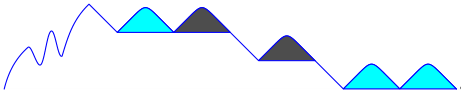
\includegraphics[width=4cm]{assets/locked-block-sketch.png}, with locked blocks darker.
\end{center}


If for every $j \leq r$, the Dyck path $X_j$ has only one block and
$X_{r+1}$ is empty, then there is no unlocked block in $u$. In this
case, the set $R_i(u)$ in the statement of \Cref{forcer_un} will be
empty. Indeed any cover relation not changing the prefix will keep the
shape of the expression~\eqref{locked_pic} fixed, so that no block
becomes unlocked and $X_0$ can never be slid.

Let us therefore from now on assume the contrary. In this case, let us
denote by $\rise_i(u)$ the element obtained from $u$ by sliding the
first block in the first $X_j$ that contains an unlocked block, up to
the height of the starting point of the last block of the previous
$X_{j-1}$ or up to the end of the prefix $p$ of $u$ if $j = 0$. In the
resulting Dyck path, there is an unlocked block inside $X_{j-1}$ if
$j > 0$.

This defines an operator $\rise_i$ that acts by sliding one unlocked block. One
will also need the operator $\rise^{(2)}_i$ defined similarly but
sliding the second available unlocked block.


\begin{lemma}
  \label{sub_forcer_un}
  Let $u \in \Dyck_n$, with a letter $0$ at position $i+1$. Let
  $v \in \Dyck_n$ such that $u \leq v$, $u$ and $v$ share a prefix of
  length $i$ and $v$ has a letter $1$ at position $i+1$. Then
  $\rise_i(u) \leq v$.
\end{lemma}

\begin{proof}
  The proof will use a decreasing induction (in the poset) on $u$
  among elements smaller than $v$ and sharing with $u$ the same prefix
  of length $i+1$.

  Since $u \leq v$, there must be an element $u'$ covering $u$ such
  that $u' \leq v$. Necessarily, $u'$ shares a prefix of length $i$
  with $u$ and $v$.

  It can happen that there is no such $u'$ sharing with $u$ a prefix
  of length $i+1$. This is the base case for the induction and it will
  just be taken care of below inside the case~\ref{sub2.1}. Otherwise, pick
  such an $u'$.

  \smallskip

  The possible such cover relations $u \leq u'$ can be classified into several types:
  \begin{enumerate}%
  \item\label{proof_lemma7.2_1} strictly inside one of the blocks of $X_k$ with $k \leq j$,
  \item\label{proof_lemma7.2_2} one block of $X_j$ is slid,
  \item\label{proof_lemma7.2_3} somewhere on the right of $X_j$.

  \end{enumerate}

  Let us first assume that there is a cover relation $u \leq u'$ of type~\eqref{proof_lemma7.2_1}
  with $u' \leq v$. In $u'$, one finds the same first unlocked block
  as in $u$. By induction, one also has $\rise_i(u') \leq v$. There
  is a sequence of cover relations $u \leq u' \leq \rise_i(u')$. But these
  cover relations commute, so that $\rise_i(u) \leq \rise_i(u')$.

  Let us now assume that there is a cover relation $u \leq u'$ of type~\eqref{proof_lemma7.2_3} with $u' \leq v$. In $u'$, one finds the same first unlocked
  block as in $u$, because this block is not the last block of
  $X_j$. By induction, one also has $\rise_i(u') \leq v$. There is a
  sequence of cover relations $u \leq u' \leq \rise_i(u')$. But these
  cover relations also commute, so that again
  $\rise_i(u) \leq \rise_i(u')$.

  There remains to assume that there is a cover relation $u \leq u'$
  of type~\eqref{proof_lemma7.2_2} with $u' \leq v$. There are three sub-cases.

  \begin{enumerate}[(2.\arabic{enumi})]
%
\setcounter{enumi}{2}
\item\label{sub2.3} 
  If the slid block $B$ is neither the
  first block nor the second block of $X_j$, then one can argue as in
  type~\eqref{proof_lemma7.2_3}, because the first unlocked block remains the
  first block of $X_j$, which is not affected.

\setcounter{enumi}{1}
\item\label{sub2.2} 
%
If the slid block $B$ is the second block of $X_j$, then either
  $X_j$ contains at least~$3$ blocks or the block $B$ is at the end of
  $u$, for otherwise $B$ is locked.  Then one can
  check directly that there is a cover relation
  $\rise_i(u) \to \rise_i(u')$. By induction, one also has $\rise_i(u') \leq v$.

  \begin{figure}[htb]
    \centering
    $u$\begin{tikzpicture}[scale=.15]
      \draw[rounded corners=1, color=black, line width=2] (4, 4) -- (5, 3) -- (6, 2) -- (7, 1) -- (8, 0) -- (9, 1) -- (10, 2) -- (11, 1) -- (12, 0) -- (13, 1) -- (14, 2) -- (15, 1) -- (16, 0) -- (17, 1);
      \draw[rounded corners=1, color=black, fill=gray, line width=2] (12, 0) -- (13, 1) -- (14, 2) -- (15, 1) -- (16, 0);
    \end{tikzpicture}$\quad\phantom{\longrightarrow}\put(-15,5){$\longrightarrow$} \quad u'$
    \begin{tikzpicture}[scale=.15]
      \draw[rounded corners=1, color=black, line width=2] (4, 4) -- (5, 3) -- (6, 2) -- (7, 1) -- (8, 0) -- (9, 1) -- (10, 2) -- (11, 1) -- (12, 2) -- (13, 3) -- (14, 2) -- (15, 1) -- (16, 0) -- (17, 1);
      \draw[rounded corners=1, color=black, fill=gray, line width=2] (11, 1) -- (12, 2) -- (13, 3) -- (14, 2) -- (15, 1) ;
    \end{tikzpicture}
    \caption{First blocks of $X_j$ for the case~\ref{sub2.2} in the proof of \Cref{sub_forcer_un}}
    \label{cas2.2}
  \end{figure}

\setcounter{enumi}{0}
\item\label{sub2.1} 
%
Assume now that the slid block $B$ is the first block of
  $X_j$. If $u' = \rise_i(u)$, the statement holds directly. This is
  what happens in the base case of the induction. Otherwise, the block
  $B$ can either be slid too high or too low compared to the exact
  height of the end of $X_{j-1}$ if $j > 0$, or too low compared to the end of the
  prefix $p$ of $u$. In both cases, it becomes (part of) a locked
  block. The existence of $v$ then forces that there is (in $u$ and $u'$) another
  unlocked block in $X_k$ for some $k \geq j$.

  If the first block $B$ of $X_j$ is slid too low in $u'$, one can
  apply repeatedly $\rise_i$ to $u'$ until this operator is sliding
  again the block $B$ itself. Let us call $u''$ the result. Starting
  from $X_k$ which contains the first unlocked block in $u'$, each
  $\rise_i$ unlocks the first block in the previous $X$. Then by
  induction, one has $u'' \leq v$. One can also see that
  $\rise_i(u) \leq u''$ by repeating on $\rise_i(u)$ all the same
  slidings performed from $u'$ to $u''$.

  The first block $B$ of $X_j$ can only be slid too high in $u'$ if
  $j > 0$, because otherwise the prefix would change. In this case,
  one can apply repeatedly $\rise_i$ to $u'$ until this operator is
  unlocking the block containing the slid block $B$ itself. Let us
  call $u''$ the result. Then by induction, one has $u'' \leq v$. Then
  one can apply the operator $\rise^{(2)}_i$ several times on
  $\rise_i(u)$ until making the slid block $B$ unlocked again. In
  other words, one replays on $\rise_i(u)$ all the sliding moves
  performed on $u'$, by replacing the action of $\rise_i$ by the
  action of $\rise^{(2)}_i$. Let us call the result $\bar{u}$. Then in $\bar{u}$,
  the block $B$ is unlocked and sliding this block (to the appropriate
  height) gives a cover relation $\bar{u} \to u''$. This implies that
  $\rise_i(u) \leq u''$.
\end{enumerate}

  In all cases, one obtains that $\rise_i(u) \leq v$.
\end{proof}

\begin{proof}
Let us now give the proof of \Cref{forcer_un}. 

One can assume that $R_i(u)$ is not empty. Let us pick any $v$ in $R_i(u)$.

Then one can iterate \Cref{sub_forcer_un}, which when applied to the
pair $(u,v)$ gives another pair $(\rise_i(u),v)$ that satisfies the
same hypotheses as long as $j > 0$. At each step, the index $j$ of
$x_j$ containing the first unlocked block in $u$ is decreased by
one. In the last step, when $j=0$, the element $\rise_i(u)$ becomes an
element $w$ of $R_i(u)$ such that $w \leq v$.

Because the construction of $w$ is an iteration of $\rise_i$ applied
to $u$, it does not depend on $v$. Therefore $w$ is smaller than any
element of $R_i(u)$. Uniqueness of such a global minimum is clear.
\end{proof}

%

For $v,w$ in $\Dyck_n$, let $M(v,w)$ be the set of Dyck paths that are
smaller than both $v$ and $w$. This set is never empty.

\begin{lemma}
  \label{meet_with_prefix}
  Let $v$ and $w$ in $\Dyck_n$ that share a prefix of length $i$. Then
  for every element $u$ in $M(v,w)$, there exists $u'$ in $M(v,w)$
  such that $u \leq u'$ and $u'$ shares a prefix of length $i$ with $v$
  and $w$.
\end{lemma}
\begin{proof}
  By induction on $i$. This is true for $i=1$, for $u'=u$. Assume now
  that $v$ and $w$ share a prefix of length $i+1$ and let $u'_i$
  be defined by induction hypothesis for the shorter common prefix of
  length $i$. If the last letter in the common prefix of length $i+1$
  is the same as the letter of $u'_i$ at position $i+1$, one can take
  $u'$ to be $u'_i$.

  Because $u'_i \in M(v,w)$, there remains only the case where the
  letter of $u'_i$ at position $i+1$ is $0$ and the last letter in the
  common prefix of length $i+1$ of $v$ and $w$ is $1$. Let us apply
  \Cref{forcer_un} to $u'_i$. The set $R_{i}(u'_i)$ is not empty as
  it contains $v$ and $w$. One can therefore take $u'$ to be its unique
  minimal element.
\end{proof}

\subsection{Proof of semilattice property}

\label{proof_semi}

Let us start with more lemmas.

Let $w$ be a Dyck path such that the $i$-th step in $w$ is $1$ and
this step does not start at height $0$.  On the right from the start
$i_0$ of $i$-th step, move on the path $w$ until meeting a point $i_1$
at the same height and followed by a $0$ step. This must happen, as
the height of $i_0$ is not zero. Between $i_0$ and $i_1$, there is in
$w$ a non-empty sequence of block-indecomposable subpaths $x_1, \dots, x_N$.

Let us define another Dyck path $\des_i(w)$ by sliding down in $w$ the
subpath $x_N$ as much as possible, namely by exchanging $x_N$ with all
the consecutive $0$ steps on its right. Then there is a cover relation
$\des_i(w) \to w$ that is sliding the subpath $x_N$ up.

\begin{lemma}
  \label{sub_force_0}
  Let $w$ be a Dyck path such that the $i$-th step in $w$ is $1$ and
  this step does not start at height $0$. Let $u \leq w$ such that the
  $i$-th step in $u$ is $0$ and $u$ and $w$ share a prefix
  of length $i - 1$. Then $u$ is smaller than $\des_i(w)$.
\end{lemma}
\begin{proof}
  The proof will be by increasing induction (in the poset) on $w$
  among elements larger than $u$ and sharing with $u$ the same prefix
  of length $i - 1$.

  Since $u \leq w$, there exists $w'$ covered by $w$ such that
  $u \leq w'$. Necessarily, $w'$ shares the same prefix of length
  $i-1$ with $u$ and $w$.

  It can happen, in the base case of the induction, that there is no
  such $w'$ that shares with $w$ a prefix of length $i$. Then it must
  be the case that $N=1$ and $w' = \des_i(w)$.

  If $w' = \des_i(w)$, the statement clearly holds.

  Because of the shared prefix, the other possible down-sliding moves
  from $w$ are of three types, according to the slid subpath $x$:
  \begin{enumerate}%
  \item\label{proof_lemma7.4_1} $x$ is inside one of the $x_j$, not ending in the final
    sequence of $0$ of $x_j$,
  \item\label{proof_lemma7.4_2} $x$ is inside one of the $x_j$, ending in the final
    sequence of $0$ of $x_j$,
  \item\label{proof_lemma7.4_3} $x$ is somewhere on the right of $x_N$.
  \end{enumerate}

  In type~\eqref{proof_lemma7.4_1}, $x_j$ is replaced by another block-indecomposable
  subpath. In type~\eqref{proof_lemma7.4_2}, if $j < N$, then $x_j$ is replaced by (split
  into) two block-indecomposable subpaths.

  Assume first that $u \leq w'$ where $w' \to w$ is of type~\eqref{proof_lemma7.4_3}. By
  induction, $u \leq \des_i(w')$. There is a chain of cover relations
  $\des_i(w') \to w' \to w$. These two cover relations commute if the slid
  subpath in the sliding move $w' \to w$ is not the first subpath after
  $x_N$. Otherwise, one can find a chain of two cover relations from
  $\des_i(w')$ to $\des_i(w)$. In all cases,
  $\des_i(w') \leq \des_i(w)$.

  Assume now that $u \leq w'$ where $w' \to w$ is of type~\eqref{proof_lemma7.4_1}. By
  induction, $u \leq \des_i(w')$. There is a chain of cover relations
  $\des_i(w') \to w' \to w$. These cover relations commute, and therefore
  $\des_i(w') \leq \des_i(w)$.

  Assume then that $u \leq w'$ where $w' \to w$ is of type~\eqref{proof_lemma7.4_2}. By
  induction, $u \leq \des_i(w')$. There is a chain of cover relations
  $\des_i(w') \to w' \to w$. If $j < N - 1$, these cover relations
  commute, and therefore $\des_i(w') \leq \des_i(w)$.

  If $j = N$, then one can apply twice the induction step to obtain that
  $u \leq \des_i(\des_i(w'))$. But $\des_i(\des_i(w')) \leq \des_i(w)$
  because one can split $x_N$ after it has been slid down.

  If $j = N-1$, one can also apply twice the induction step, to get
  that $u \leq \des_i(\des_i(w'))$. One then checks that
  $\des_i(\des_i(w')) \leq \des_i(w)$ holds also in this case, by just
  one cover relation.

  One therefore deduces the statement in all cases.
\end{proof}

Keeping the same notations, let $s_i(w)$ denote $\des_i^N(w)$, the
image of $w$ under the $N$-times iteration of the application
$\des_i$.

\begin{lemma}
  \label{force_0}
  Let $w$ be a Dyck path such that the $i$-th step in $w$ is $1$ and
  this step does not start at height $0$. Let $S_i(w)$ be the set
  of all Dyck paths $u$ such that $u \leq w$, the $i$-th letter of $u$
  is $0$ and $u$ and $w$ share the same prefix before the $i$-th letter.
  Then $s_i(w)$ is the unique maximal element of $S_i(w)$.
\end{lemma}
\begin{proof}
  First note that $s_i(w)$ is indeed in $S_i(w)$.

  Let $u$ be an element of $S_i(w)$. One can apply \Cref{sub_force_0}
  to the pair $(u,w)$ to get another pair $(u, w')$ where
  $w'=\des_i(w)$. Either $w' = s_i(w)$, or this new pair satisfies
  again the hypotheses of \Cref{sub_force_0}. One can therefore repeat
  this exactly $N$ times, until reaching the pair $(u,s_i(w))$. In
  particular, $u \leq s_i(w)$.
\end{proof}


\begin{theorem}
  The poset $(\Dyck_n, \sm)$ is a meet-semilattice.
\end{theorem}
\begin{proof}
  Let $v$ and $w$ be two Dyck paths, and let us look for their
  meet. One can assume that $v$ and $w$ are not equal.

  Start from the left, until meeting a difference between $v$ and
  $w$. Let $i$ be the last common point. One can assume that $w$ is
  above $v$ just after the point $i$, by exchanging $v$ and $w$ if
  necessary. Note that the height of $i$ cannot be zero.

  One can therefore apply \Cref{force_0} to $w$ for the step after
  position $i$, and obtain an element $w'$ which is maximal among all
  elements smaller than $w$ that share the same prefix followed by
  the letter $0$.

  This gives a new pair of elements $(v,w')$ with $w' \leq w$. Let us
  prove that $M(v,w) = M(v,w')$. The inclusion $M(v,w') \subseteq
  M(v,w)$ is clear because $w' \leq w$.

  Conversely, let $u$ be an element of $M(v,w)$. Using
  \Cref{meet_with_prefix}, one can find $u'$ in $M(v,w)$ with $u \leq
  u'$ and $u'$ share the common prefix of $v$ and $w$. Note that the
  first letter after the common prefix in $u'$ is $0$, because $u'
  \leq v$. It therefore follows from the definition of $w'$ that $u'
  \leq w'$.

  Hence $M(v,w) = M(v,w')$, and the common prefix of $v$ and $w'$ is
  strictly longer. Therefore iterating this whole procedure on pairs
  of Dyck paths ends at a common Dyck path $z$, that is smaller than
  $v$ and $w$ and such that $M(z,z) = M(v,w)$. This $z$ is therefore
  the meet of $v$ and $w$.
\end{proof}
\begin{thebibliography}{99}
\bibitem[1]{bpr} Bergeron, François; Préville-Ratelle, Louis-François Higher trivariate diagonal harmonics via generalized Tamari posets, J. Comb., Volume 3 (2012) no. 3, pp. 317-341.
\bibitem[2]{berbon} Bernardi, Olivier; Bonichon, Nicolas Intervals in Catalan lattices and realizers of triangulations, J. Comb. Theory, Ser. A, Volume 116 (2009) no. 1, pp. 55-75.
\bibitem[3]{mbmpr} Bousquet-Mélou, Mireille; Fusy, Éric; Préville-Ratelle, Louis-François The number of intervals in the m-Tamari lattices, Electron. J. Comb., Volume 18 (2011) no. 2, Paper no. P31, 26 pages.
\bibitem[4]{mbmj} Bousquet-Mélou, Mireille; Jehanne, Arnaud Polynomial equations with one catalytic variable, algebraic series and map enumeration, J. Comb. Theory, Ser. B, Volume 96 (2006) no. 5, pp. 623-672.
\bibitem[5]{chap_slc} Chapoton, Frédéric Sur le nombre d’intervalles dans les treillis de Tamari, Sémin. Lothar. Comb., Volume 55 (2005/07), Paper no. Art. B55f, 18 pages.
\bibitem[6]{chap_cats} Chapoton, Frédéric On the categories of modules over the Tamari posets, Associahedra, Tamari lattices and related structures (Prog. Math.), Volume 299, Birkhäuser/Springer, Basel, 2012, pp. 269-280.
\bibitem[7]{fang3} Fang, Wenjie Planar triangulations, bridgeless planar maps and Tamari intervals, Eur. J. Comb., Volume 70 (2018), pp. 75-91.
\bibitem[8]{fang2} Fang, Wenjie A trinity of duality: non-separable planar maps, \(\beta\)(1,0)-trees and synchronized intervals, Adv. Appl. Math., Volume 95 (2018), pp. 1-30.
\bibitem[9]{fangpr} Fang, Wenjie; Préville-Ratelle, Louis-François The enumeration of generalized Tamari intervals, Eur. J. Comb., Volume 61 (2017), pp. 69-84.
\bibitem[10]{freese} Freese, Ralph; Ježek, Jaroslav; Nation, James B. Free lattices, Math. Surv. Monogr., 42, American Mathematical Society, Providence, RI, 1995, viii+293 pages.
\bibitem[11]{tamari_friedman} Friedman, Haya; Tamari, Dov Problèmes d’associativité: Une structure de treillis finis induite par une loi demi-associative, J. Comb. Theory, Volume 2 (1967), pp. 215-242.
\bibitem[12]{gratzer} Grätzer, George Lattice theory: foundation, Birkhäuser/Springer Basel AG, Basel, 2011, xxx+613 pages.
\bibitem[13]{flipflop} Ladkani, Sefi Universal derived equivalences of posets of tilting modules (2007) (\url{https://arxiv.org/abs/0708.1287}).
\bibitem[14]{lenzing} Lenzing, Helmut Coxeter transformations associated with finite-dimensional algebras, Computational methods for representations of groups and algebras (Essen, 1997) (Prog. Math.), Volume 173, Birkhäuser, Basel, 1999, pp. 287-308.
\bibitem[15]{loday} Loday, Jean-Louis The diagonal of the Stasheff polytope, Higher structures in geometry and physics (Prog. Math.), Volume 287, Birkhäuser/Springer, New York, 2011, pp. 269-292.
\bibitem[16]{MTTV} Masuda, Naruki; Thomas, Hugh; Tonks, Andy; Vallette, Bruno The diagonal of the associahedra (2019) (\url{https://arxiv.org/abs/1902.08059}).
\bibitem[17]{tamari_festschrift} Associahedra, Tamari lattices and related structures (Müller-Hoissen, Folkert; Pallo, Jean Marcel; Stasheff, Jim, eds.), Prog. Math., 299, Birkhäuser/Springer, Basel, 2012, xx+433 pages (Tamari memorial Festschrift).
\bibitem[18]{pallo} Pallo, Jean Marcel Right-arm rotation distance between binary trees, Inf. Process. Lett., Volume 87 (2003) no. 4, pp. 173-177.
\bibitem[19]{rivera_san} Rivera, Manuel; Saneblidze, Samson A combinatorial model for the free loop fibration (2017) (\url{https://arxiv.org/abs/1712.02644}).
\bibitem[20]{rognerud} Rognerud, Baptiste Exceptional and modern intervals of the Tamari lattice (2018) (to appear in Sémin. Lothar. Comb.).
\bibitem[21]{san_arxiv} Saneblidze, Samson The bitwisted Cartesian model for the free loop fibration, Topology Appl., Volume 156 (2009) no. 5, pp. 897-910.
\bibitem[22]{san_note} Saneblidze, Samson On the homology theory of the closed geodesic problem, Rep. Enlarged Sess. Semin. I. Vekua Inst. Appl. Math., Volume 25 (2011), pp. 113-116.
\bibitem[23]{tutte} Tutte, William T. A census of planar maps, Can. J. Math., Volume 15 (1963), pp. 249-271.
\end{thebibliography}
\end{document}
